\documentclass[11pt,aspectratio=43]{beamer}
\usepackage[utf8]{inputenc}
\usepackage{amsmath, amsfonts, amssymb, amsthm}
\usepackage[T1]{fontenc}
\usepackage{lmodern}
\usepackage{xcolor}
\usepackage{setspace}
\usepackage{booktabs}
\usepackage{multirow}
\usepackage{graphicx}
\usepackage{tikz}
% \usetikzlibrary{decorations}
\usetikzlibrary{decorations.pathreplacing}
\usepackage{ulem}
\usepackage{hyperref}
\usepackage{booktabs}
\usepackage{babel}
\usepackage{makecell}
\usepackage[para,online,flushleft]{threeparttable}
\usepackage{pdfpages}
\usepackage{tcolorbox}
\usepackage{bm}
\usepackage{appendixnumberbeamer}
\usepackage{natbib}
\usepackage{caption}
\captionsetup[figure]{labelformat=empty}% redefines the caption setup of the figures environment in the beamer class.
\usetheme[compress]{Boadilla}
\usecolortheme{default}
\useoutertheme{miniframes}
\usefonttheme[onlymath]{serif}

\newcommand{\jump}[2]{\hyperlink{#1}{\beamerbutton{#2}}}
\newcommand{\orange}[1]{\textcolor{orange}{#1}}
\newcommand{\red}[1]{\textcolor{red}{#1}}

\setbeamertemplate{itemize item}{\raisebox{0.1em}{\scalebox{0.7}{$\blacksquare$}}}
\setbeamertemplate{itemize subitem}[circle]
\setbeamertemplate{itemize subsubitem}{--}
\setbeamercolor{itemize item}{fg=black}
\setbeamercolor{itemize subitem}{fg=black}
\setbeamercolor{itemize subsubitem}{fg=black}
\setbeamercolor{item projected}{bg=darkgray,fg=white}
\definecolor{blue}{rgb}{0.2, 0.2, 0.7}
\setbeamercolor{alerted text}{fg=blue}
\setbeamertemplate{enumerate items}[circle]


\setbeamertemplate{headline}{}

%==========================================
\let\olditemize=\itemize
\let\endolditemize=\enditemize
\renewenvironment{itemize}{\olditemize \itemsep1em}{\endolditemize}
\let\oldenumerate=\enumerate
\let\endoldenumerate=\endenumerate
\renewenvironment{enumerate}{\oldenumerate \itemsep1em}{ \endoldenumerate}

\DeclareMathOperator*{\argmax}{\arg\!\max}
\DeclareMathOperator*{\E}{\mathbb{E}}
\DeclareMathOperator*{\var}{\rm Var}
\DeclareMathOperator*{\cov}{\rm Cov}

\theoremstyle{definition}
\newtheorem{assume}{Assumption}
\newtheorem{lem}{Lemma}
\newtheorem{proposition}{Proposition}
\newtheorem{thm}{Theorem}
\newtheorem{corol}{Corollary}

\begin{document}
    \title[Lecture 6]{Lecture 6 \\ Numerical Example}
    \author[Hui-Jun Chen]{Hui-Jun Chen}
    \institute[OSU]{The Ohio State University}
    % \date{\today}
    \date[\today]{\today \\ Credit: Kyle Dempsey}
    \setbeamertemplate{navigation symbols}{}
    \setstretch{1.2}

%-------------------------------------------------------
{
%	\usebackgroundtemplate{\includegraphics[width=1\paperwidth]{../EveningSky_cropped_edit43_bright.jpg}}
    \begin{frame}
% \vspace{3em}
        \centering
%		{\footnotesize 	ECON 4002 Intermediate Macroeconomic Theory}
        \maketitle
% \vspace{-1.5em}
% \centering
% \includegraphics[width=0.55\linewidth]{Pictures/houses.jpeg}


    \end{frame}
}

% -------------------------------------------
\setbeamertemplate{headline}
{
\setbeamercolor{section in head/foot}{fg=black, bg=white}
\vskip1em \tiny \insertsectionnavigationhorizontal{1\paperwidth}{\hspace{0.50\paperwidth}}{}
}
%------------------------------------------

\begin{frame}{Overview: Lecture 4 - 7}
\label{slide:Overview__Lecture_4_7}

\begin{center}
Provide \alert{micro-foundation} for the \alert{macro implication} (\alert{Lucas critique})
\end{center}

\begin{itemize}
    \item \textbf{Representative Consumer}:
    \begin{itemize}
        \item Lecture 4: \alert{preference}, \alert{constraints}
        \item Lecture 5: \alert{optimization}, \alert{application}
        \item Lecture 6: Numerical Examples
    \end{itemize}
    \item \textbf{Representative Firm}:
    \begin{itemize}
        \item Lecture 7: \alert{production}, \alert{optimization}, \alert{application}
    \end{itemize}
\end{itemize}
\end{frame}

\section{Optimization Basic}
\label{sec:Optimization_Basic}

\begin{frame}{$1$ Variable}
\label{slide:_1__Variable}
    \begin{columns}
        \begin{column}{0.6\textwidth}
            \begin{figure}
                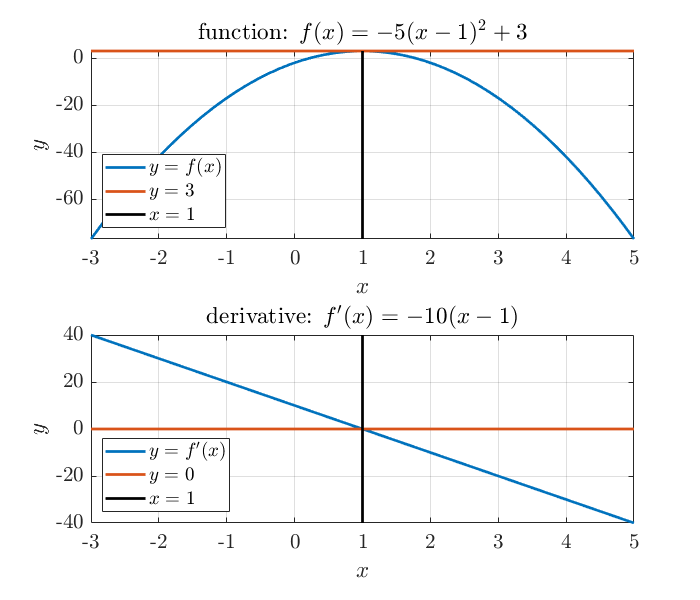
\includegraphics[width=\textwidth]{./figures/1Var.png}
            \end{figure}
        \end{column}
        \begin{column}{0.4\textwidth}
            In general, want to solve $\max_{x} f( x )$
            \begin{itemize}
                \item find ``peak'' of function
                \item at peak, slope is $ 0 $
                \item \textbf{First order condition} (FOC) is when the 1st order derivative, i.e., the slope is $ 0 $:
                %
                \begin{equation*}
                   f'( x^{*} ) = 0
                ,\end{equation*}
                %
                where $ x^{*} $ is the peak
            \end{itemize}
        \end{column}
    \end{columns}
\end{frame}

\begin{frame}{$2$ Variables}
\label{slide:_2__Variables}
    \begin{columns}
        \begin{column}{0.6\textwidth}
            \begin{figure}
                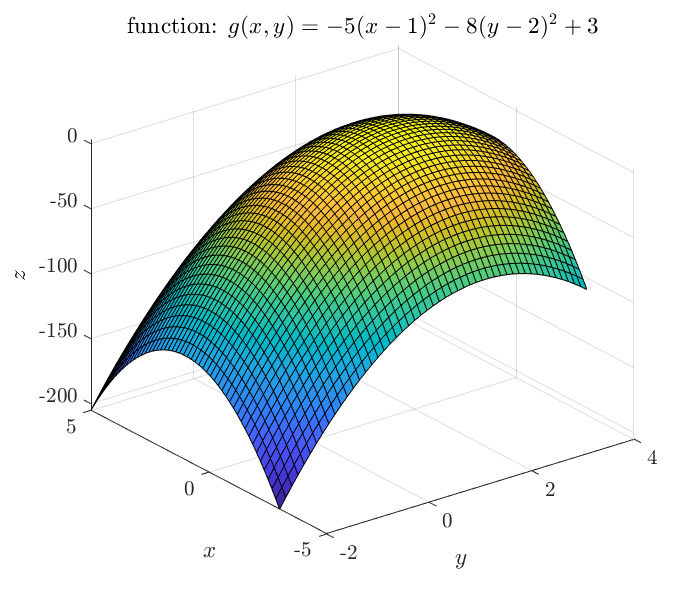
\includegraphics[width=\textwidth]{./figures/2Var.png}
            \end{figure}
        \end{column}
        \begin{column}{0.4\textwidth}
            In general, want to solve $\max_{x, y} g( x, y )$
            \begin{itemize}
                \item at peak, slope is $ 0 $ \alert{in both directions}, i.e., the FOC\alert{s} are
                %
                \begin{equation*}
                    \begin{split}
                        D_{x}g( x^{*}, y^{*} )
                            & = 0
                        \\
                        D_{y}g( x^{*}, y^{*} )
                            & = 0
                        \\
                    \end{split}
                ,\end{equation*}
                %
                where the bundle $ (x^{*}, y^{*}) $ is the peak
                \item Hard for my brain to process 3-D graph...\alert{resolution}?
            \end{itemize}
        \end{column}
    \end{columns}

\end{frame}

\begin{frame}{Visualizing 3-D function on 2-D plane}
\label{slide:Visualizing_3_D_function_on_2_D_plane}

    \begin{columns}
        \begin{column}{0.5\textwidth}
            \begin{figure}
                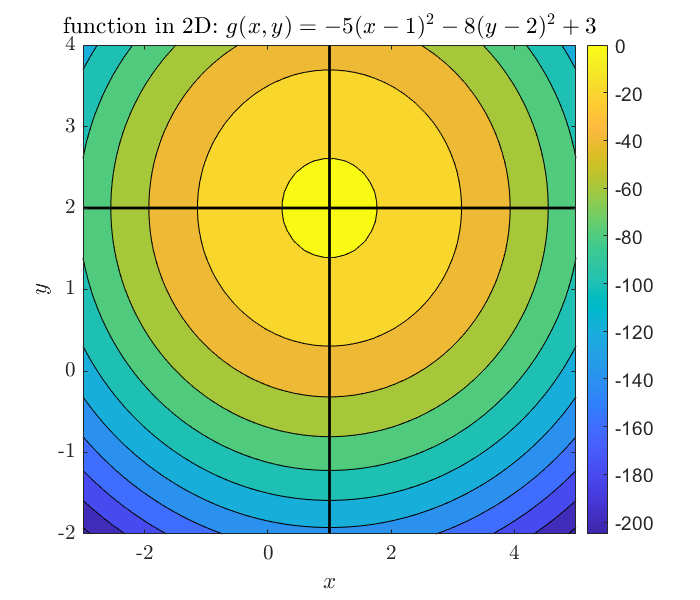
\includegraphics[width=\textwidth]{./figures/2VarContours.png}
            \end{figure}
        \end{column}
        \begin{column}{0.5\textwidth}
            \begin{itemize}
                \item \textbf{Contours}:``standing'' at the peak and look down
                \begin{itemize}
                    \item e.g. \alert{\href{https://www.alltrails.com/}{map on Alltrails}}
                \end{itemize}
                \item Fix the level of $ g = -20 $ (a \alert{horizontal slice} of 3-D figure)
                \item Find $ x $ and $ y $ such that
                %
                \begin{equation*}
                     -20 = -5( x-1 )^{2} - 8( y-2 )^{2} + 3
                \end{equation*}
                %
                \item repeat for any value of $ g $
                \item \textbf{Exactly where indifference curve came from!}
            \end{itemize}
        \end{column}
    \end{columns}
\end{frame}

\begin{frame}{Solving $2$ Variables Optimizations}
\label{slide:Solving__2__Variables_Optimizations}

    \begin{columns}
        \begin{column}{0.5\textwidth}
            \begin{figure}
                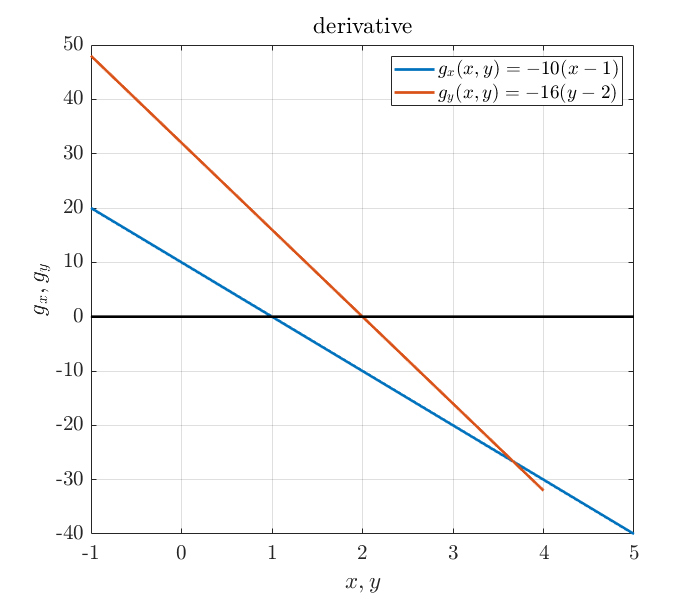
\includegraphics[width=\textwidth]{./figures/2VarOptimize.png}
            \end{figure}
        \end{column}
        \begin{column}{0.5\textwidth}
            %
            \begin{equation*}
                  \begin{split}
                        D_{x} g( x^{*}, y^{*} )
                            & = -10( x-1 ) = 0
                        \\
                        D_{y} g( x^{*}, y^{*} )
                            & = -16( y-2 ) = 0
                        \\
                  \end{split}
            \end{equation*}
            \begin{itemize}
                \item \alert{Intersection} between $ 0 $ and line is the solution.
                \item For other functional form, $ D_{x} g( x, y ) $ can depend on $ y $, and $ D_{y}g( x, y ) $ can depend on $ x $
                \item May have constraints on the relationship between $ x $ and $ y $
            \end{itemize}
        \end{column}
    \end{columns}
\end{frame}

\section{Consumer Example}
\label{sec:Consumer_Example}

\begin{frame}{Utility Function in 3-D}
\label{slide:Utility_Function_in_3_D}
    \begin{center}
        Here $ a = b = 1 $, \alert{where is the peak?}
    \end{center}
    \begin{columns}
        \begin{column}{0.7\textwidth}
            \begin{figure}
                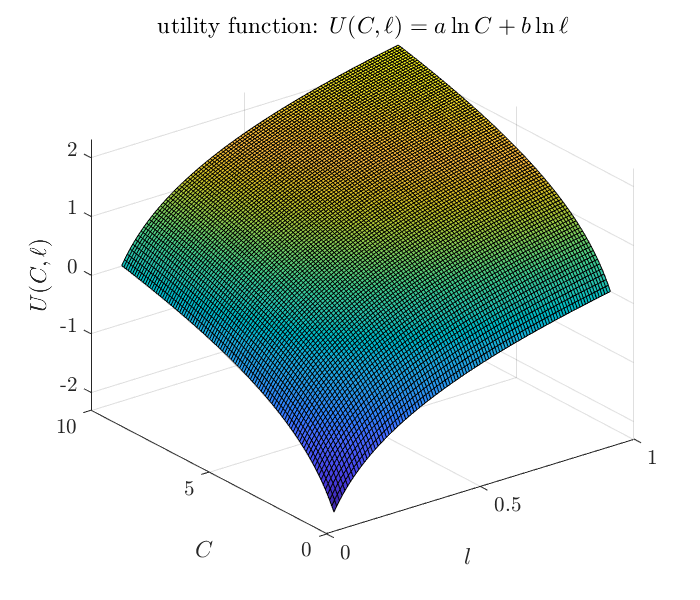
\includegraphics[width=\textwidth]{./figures/Utility.png}
            \end{figure}
        \end{column}
        \begin{column}{0.3\textwidth}
            \begin{itemize}
                \item Seems like to be at $ C^{*} = 10 $ and $ l^{*} = 1 $
                \item Recall \alert{monotonicity}: more is better!
                \item What \alert{stops} the consumer from choose $ ( C, l ) = ( 10, 1 ) $?
            \end{itemize}
        \end{column}
    \end{columns}
\end{frame}

\begin{frame}{Utility Function + Budget Set in 3-D}
\label{slide:Utility_Function___Budget_Set_in_3_D}
    Let $ w = 10 $ and $ h = 1 $, and the gray surface represents the \alert{border} of the budget set.
    \begin{columns}
        \begin{column}{0.6\textwidth}
            \begin{figure}
                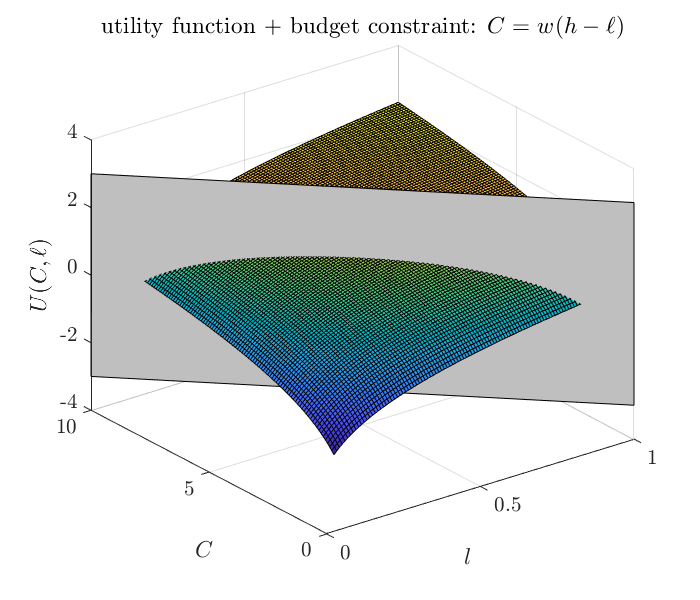
\includegraphics[width=\textwidth]{./figures/UtilityBudget.png}
            \end{figure}
        \end{column}
        \begin{column}{0.4\textwidth}
            \begin{itemize}
                \item Consumers have to choose $ ( C, l ) $ bundles \alert{inside the budget set}
                \begin{itemize}
                    \item $ ( C, l ) = ( 10, 1 ) $ is \alert{outside} of the budget set $ \Rightarrow  $ not feasible
                \end{itemize}
                \item \textbf{Binding budget constraint}: candidates for optimal are points in gray
                \item Which one?
            \end{itemize}
        \end{column}
    \end{columns}
\end{frame}

\begin{frame}{Collapsing 3-D Problem into 2-D: Slice}
\label{slide:Collapsing_3_D_Problem_into_2_D_Slice}
\begin{center}
    How? Binding budget constraint!
\end{center}
\begin{columns}
    \begin{column}{0.5\textwidth}
        \begin{figure}
            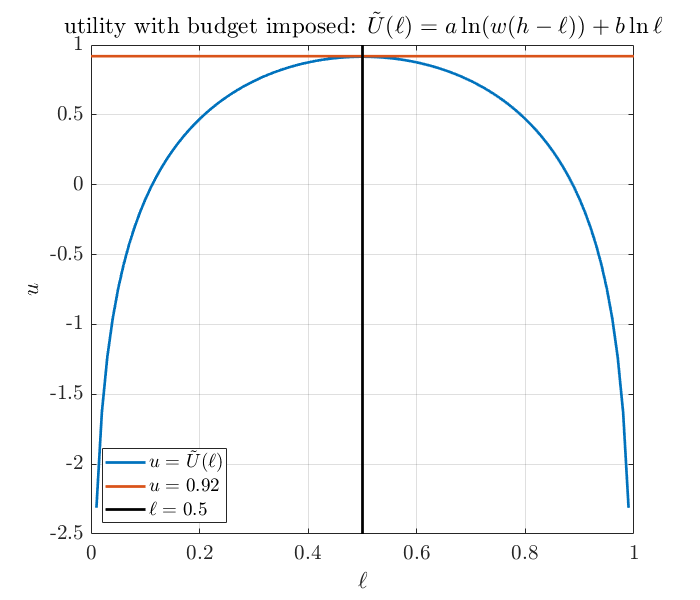
\includegraphics[width=\textwidth]{./figures/UtilityBudget2C.png}
        \end{figure}
    \end{column}
    \begin{column}{0.5\textwidth}
        %
        \begin{align*}
            \text{Binding:} \quad
                & C = w ( h-l )
            \\
                & U( C, l ) = a \ln C + b \ln l
            \\
            \text{Plug in:} \quad
                & \tilde{U}( l ) = a \ln ( w( h-l ) ) + b \ln l
            \\
            \text{FOC:} \quad
                & D_{l}\tilde{U}( l ) = 0
            \\
                & a \frac{-w}{w( h-l )} + b \frac{1}{l} = 0
            \\
                & \frac{a}{h-l} = \frac{b}{l}
            \\
                & l = \frac{b}{a+b} h
        \end{align*}
        $ l = 0.5 $, let $ C =  5$, $ u = 0.91629... $
    \end{column}
\end{columns}
\end{frame}

\begin{frame}{Collapsing 3-D Problem into 2-D: Contours}
\label{slide:Collapsing_3_D_Problem_into_2_D__Contours}
Recall \alert{contours}, for any utility level $ u $, $ u = a \ln C + b \ln l $ $ \Rightarrow  $ $ C = e^{ \frac{u - b \ln l}{a}} $
\begin{columns}
    \begin{column}{0.6\textwidth}
        \begin{figure}
            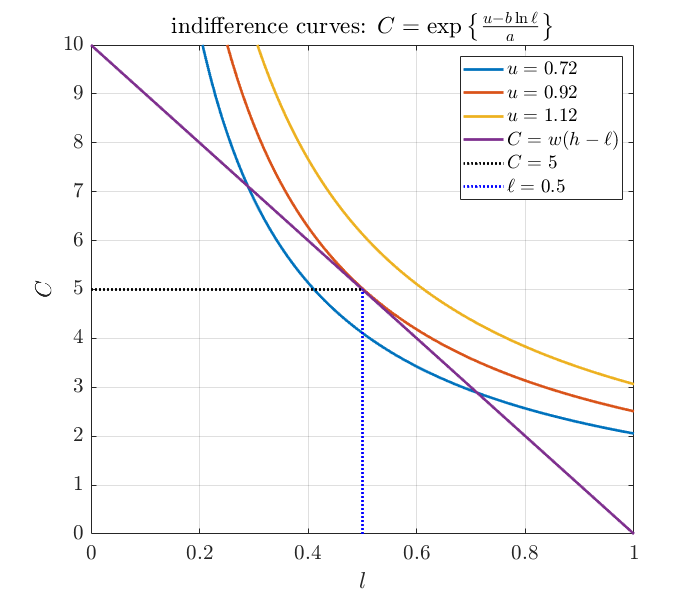
\includegraphics[width=\textwidth]{./figures/UtilityBudget2DContour.png}
        \end{figure}
    \end{column}
    \begin{column}{0.4\textwidth}
        \begin{itemize}
            \item \alert{What is the highest $ u $ feasible given budget constraint}?
            % \item Similar to last slide: plug in $ C = w( h-l ) $ and maximize w.r.t. $ l $
            \item Or push up IC (increase $ u $) such that IC is tangent to budget line:
                %
                \begin{align*}
                   - MRS_{l, C}
                       & = -w
                   \\
                    \frac{b C}{a l} = \frac{b w ( h-l )}{a l}
                        & = w
                    \\
                    l
                        & = \frac{b}{a+b}h
                    \\
                \end{align*}
                %
        \end{itemize}
    \end{column}
\end{columns}

\end{frame}

\begin{frame}{2-D versions: Pros and Cons}
\label{slide:2_D_versions__Pros_and_Cons}
    Both 2-D formulations are delivering the same answer.
    \begin{enumerate}
        \item Slice: $ 1 $ variable optimization problem, $ x $-axis: $ l $, $ y $-axis: $ u $
        \begin{itemize}
            \item \textbf{Straightforward}: operate on $ ( l, u ) $ plane, good for problem solving
            \item \textbf{General}: can collapse higher dimension problem
            \item \textbf{Cons}: lack of trade off between $ C $ and $ l $ $ \Rightarrow  $ \alert{economcis intuition}
        \end{itemize}
        \item Contours: $ 2 $ variable optimization problem, $ x $-axis: $ l $, $ y $-axis: $ C $
        \begin{itemize}
            \item \textbf{Intuitive}: direct trade off between $ C $ and $ l $ through $ MRS_{l, C} $
            \item \textbf{Cons:} harder to solve and to generalize to higher dimension
        \end{itemize}
    \end{enumerate}

\end{frame}

\section{Experiments}
\label{sec:Experiments}

\begin{frame}{Review: Models from Last Lecture}
\label{slide:Review__Models_from_Last_Lecture}
    \begin{enumerate}
        \item Utility function: $ U( C, l ) = a \ln C + b \ln l $
        \item Budget constraint: $ C \le w( h-l ) + \pi - T $
        \item After-tax dividend: $ x = \pi - T $
        \item wage rate: $ w $
    \end{enumerate}
    \begin{itemize}
        \item \textbf{Benchmark}: in section \nameref{sec:Consumer_Example}
        \item \textbf{Experiment 1}: increase in after-tax dividend: $ x_{1} > x_{0} $
        \item \textbf{Experiment 2}: increase wage rate: $ w_{2} > w_{0} $
    \end{itemize}
\end{frame}

\begin{frame}{Solve for Benchmark Case}
\label{slide:Solve_for_Benchmark_Case}
\begin{itemize}
    \item \textbf{Marginal utilities}: $ D_{C} U( C, l ) = \frac{a}{C} $; $ D_{l} U( C, l ) = \frac{b}{l} $.
    \item \textbf{Binding budget constraint}: $ C = w( h-l ) + \pi - T $
    \item \textbf{Optimality}: $ MRS_{l, C} = w $ $ \Rightarrow  $ $ \frac{D_{l}U( C, l )}{D_{C}U( C, l )} = w $ $ \Rightarrow  $ $ w = \frac{bC}{al} $
\end{itemize}
Plug binding budget constraints into optimality and solve for $ l $:
%
\begin{align}
        & w = \frac{b ( w( h-l ) + x )}{al}
    \\
    \Rightarrow \quad
        & w a l = b( w( h-l ) + x )
    \\
    \Rightarrow \quad
        & w a l = bwh - bwl + bx
    \\
    \Rightarrow \quad
        & ( a+b ) wl = bwh + bx
    \\
    \Rightarrow \quad
        & l = \frac{b}{a+b} \left( h + \frac{x}{w} \right)
\end{align}
%
\end{frame}

\begin{frame}{Solve for Benchmark Case (Cont.)}
\label{slide:Solve_for_Benchmark_Case__Cont__}
    Solve for $ C $, we get
    %
    \begin{align}
            & l = \frac{b}{a+b} \left( h + \frac{x}{w} \right) \Rightarrow \red{w l = \frac{b}{a+b} \left( w h + x \right)}
        \\
            & C = w( h-l ) + \pi - T = w( h-l ) + x
        \\
        \Rightarrow \quad
            & C = w \left[
                h - \frac{b}{ a+b}
                \left( h + \frac{x}{w} \right)
            \right] + x
        \\
        \Rightarrow \quad
            & C = wh - \frac{b}{a+b} \left(
                wh + x
            \right) + x
        \\
        \Rightarrow \quad
            & C = \frac{a}{a+b} wh + \frac{a}{a+b} x
        \\
        \Rightarrow \quad
            & \red{C = \frac{a}{a+b} \left( wh + x \right)}
    \end{align}
    %
    \textbf{Property for this utility function}: consumer ``\alert{split}'' fixed share of ``\alert{wealth}'': $ wl = s( wh + x ) $, and $ C = ( 1-s ) ( wh + x ) $.
\end{frame}

\begin{frame}{Solve for Experiment 1: $ x \uparrow  $}
\label{slide:Solve_for_Experiment_1____x__uparrow_______}
$ (l_{0}, C_{0}, x_{0} )$: benchmark value;
$ (l_{1}, C_{1}, x_{1} )$: experiment 1 value.

With pure income effect, \alert{no change in real wage}: $ w_{1} = w_{0} = w$

The difference between experiment 1 and benchmark case is
%
\begin{align}
    l_{1} - l_{0}
        & = \frac{b}{a+b} \left( h + \frac{x_{1}}{w} \right)
          - \frac{b}{a+b} \left( h + \frac{x_{0}}{w} \right)
    \\
        & = \frac{b}{a+b} \left( \frac{x_{1}}{w} - \frac{x_{0}}{w} \right)
    \\
        & = \frac{b}{(a+b)w} \left( x_{1} - x_{0} \right) > 0
    \\
    C_{1} - C_{0}
        & = \frac{a}{a+b} \left( wh + x_{1} \right)
          - \frac{a}{a+b} \left( wh + x_{0} \right)
    \\
        & = \frac{a}{a+b} \left( x_{1} - x_{0} \right) > 0
\end{align}
%
Namely, with pure income effect, \alert{both leisure and consumption increases}.
\end{frame}

\begin{frame}{Solve for Experiment 1: Graphical Intuition}
\label{slide:Solve_for_Experiment_1__Graphical_Intuition}
    $ w_{1} = w_{0} = 10 $; $ x_{1} = 1 > x_{0} = 0 $
    \begin{columns}
        \begin{column}{0.5\textwidth}
            \begin{figure}
                \caption{Both leisure and consumption are higher}
                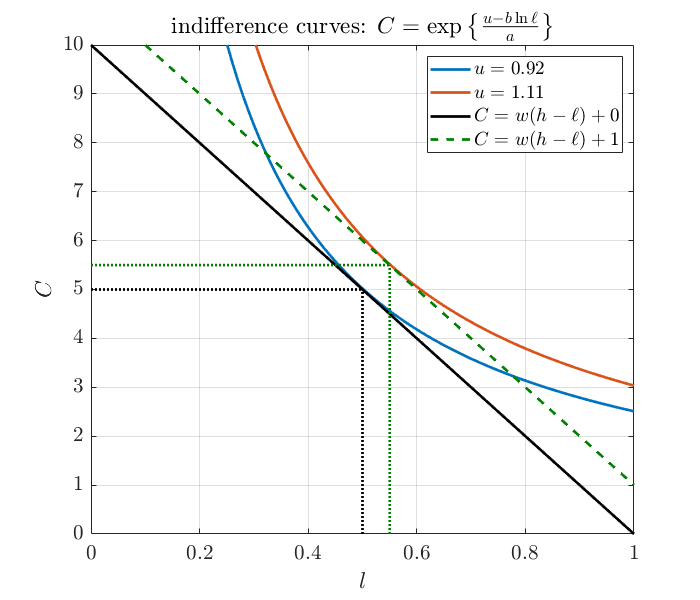
\includegraphics[width=\textwidth]{./figures/Experiment1IC.png}
            \end{figure}
        \end{column}
        \begin{column}{0.5\textwidth}
            \begin{figure}
                \caption{Budget constraint is ``\alert{eased}''}
                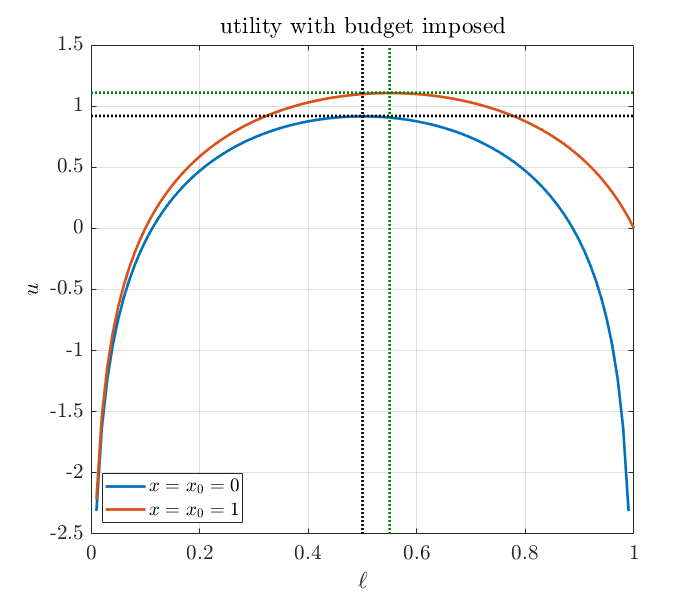
\includegraphics[width=\textwidth]{./figures/Experiment1Utility.png}
            \end{figure}
        \end{column}
    \end{columns}
\end{frame}

\begin{frame}{Solve for Experiment 2: $ w \uparrow $}
\label{slide:Solve_for_Experiment_2____w__uparrow__}
$ (l_{0}, C_{0}, x_{0} )$: benchmark value;
$ (l_{2}, C_{2}, x_{2} )$: experiment 2 value.

With both income and substitution effects, analysis is complicated:
%
\begin{align}
    l_{2} - l_{0}
        & = \frac{b}{a+b} \left( h + \frac{x_{2}}{w_{2}} \right)
          - \frac{b}{a+b} \left( h + \frac{x_{0}}{w_{0}} \right)
    \\
        & = \frac{b}{a+b} \left( \frac{x_{2}}{w_{2}} - \frac{x_{0}}{w_{0}} \right) \red{ \gtreqqless 0}
    \\
    C_{2} - C_{0}
        & = \frac{a}{a+b} \left( w_{2}h + x_{2} \right)
          - \frac{a}{a+b} \left( w_{0}h + x_{0} \right)
    \\
        & = \frac{a}{a+b} \left(
            h( w_{2} - w_{0} ) + ( x_{2} - x_{0} )
        \right) \alert{> 0}
\end{align}
%
Although the consumption is certainly increasing, \alert{the change in leisure is uncertain} $ \Rightarrow  $ need \alert{numerical solution} (put numbers in).

\end{frame}

\begin{frame}{Solve for Experiment 2: $ w \uparrow $ (Cont.)}
\label{slide:Solve_for_Experiment_2____w__uparrow____Cont__}
    Let $ w_{2} = 15 > w_{0} = 10 $; $ x_{2} = x_{0} = 0 $.
    \begin{align}
        l_{2} - l_{0}
            & = \frac{b}{a+b} \left( \frac{x_{2}}{w_{2}} - \frac{x_{0}}{w_{0}} \right)
                = \frac{b}{a+b} \left( \frac{0}{15} - \frac{0}{10} \right) = 0
    \end{align}
    Leisure remain the same.

    Compare with experiment 1, $ w_{2} = 15 > w_{1} = 10 $; $ x_{2} = 0 < x_{1} = 1$; $ h = 1 $:
    \begin{align}
        l_{2} - l_{1}
            & = \frac{b}{a+b} \left( \frac{x_{2}}{w_{2}} - \frac{x_{1}}{w_{1}} \right) = \frac{b}{a+b} \left( \frac{0}{15} - \frac{1}{10} \right) < 0
        \\
        C_{2} - C_{1}
            & = \frac{a}{a+b} \left( h( w_{2} - w_{1} ) + ( x_{2} - x_{1} ) \right)
        \\
            & = \frac{a}{a+b} ( 1 ( 15 - 10 ) + (0 - 1) ) > 0
    \end{align}

\end{frame}

\begin{frame}{Experiment 2 v.s. Benchmark: Graphical Intuition}
\label{slide:Solve_for_Experiment_2__Graphical_Intuition}
    \begin{columns}
        \begin{column}{0.5\textwidth}
             \begin{figure}
                \caption{Total Effect}
                 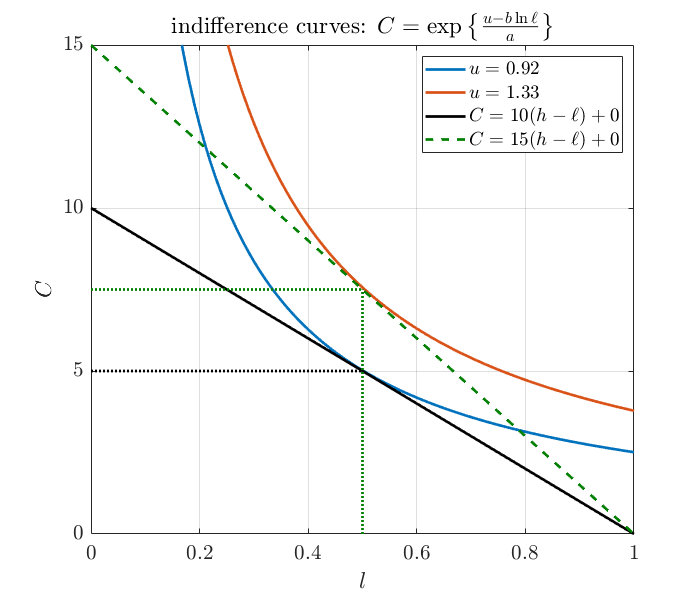
\includegraphics[width=\textwidth]{./figures/Experiment2IC.png}
             \end{figure}
        \end{column}
        \begin{column}{0.5\textwidth}
             \begin{figure}
                \caption{Income and Substitution Effect}
                 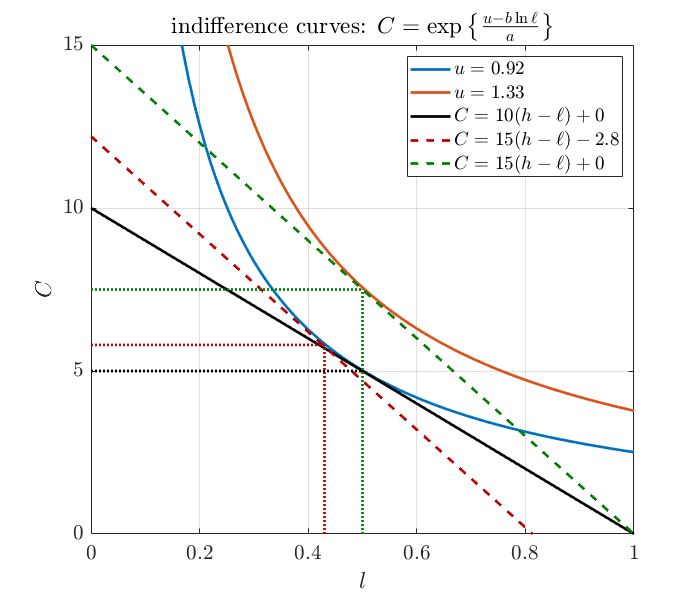
\includegraphics[width=\textwidth]{./figures/Experiment2IncomeSubEffect.png}
             \end{figure}
        \end{column}
    \end{columns}
\end{frame}

\end{document}
